%%%%%%%%%%%%%
%                                 %
%  Beamer Template  % 
%   with: handout        %
%   and: twoup print    %
%                                 %
%%%%%%%%%%%%%
\newif\ifhandout
\newif\iftwoup
% \handouttrue		% uncomment to get handouts; default is false; 		links are active
% \twouptrue  		% uncomment to get 'two-up' handouts; default is false;	links are dead
\ifhandout
% setup for printed handouts: no overlays, print 2 up, grey background
\documentclass[10pt,handout,hyperref={colorlinks=true,linkcolor=blue,citecolor=citelink,urlcolor=gray}]{beamer}
	\iftwoup
	\usepackage{pgfpages}
	\pgfpagesuselayout{2 on 1}[letterpaper,border shrink=5mm]
	\mode<handout>{\setbeamercolor{background canvas}{bg=black!5}}
	\fi
\else
% setup for class presentation slides
\documentclass[10pt,hyperref={colorlinks=true,linkcolor=blue,citecolor=citelink,urlcolor=gray}]{beamer}
\fi

\usepackage{mathptmx}
\usefonttheme{professionalfonts}
\usepackage{amsmath,amssymb}% ,amscd}
\usepackage{multicol}

\usetheme{Singapore}
\usecolortheme{rose}
\setbeamertemplate{blocks}[rounded][shadow=true]
\setbeamertemplate{navigation symbols}{}

\newtheorem{proposition}{Proposition}
\newtheorem{experiment}{Experiment}
\newtheorem{project}{Project}
\newtheorem{exercise}{Exercise}
\newtheorem{exercises}{Exercises}

\title{Analytic Hierarchy Process}
\author{\href{http://www.mathsci.appstate.edu/~wmcb/}{Wm C Bauldry}}
\institute{MAT 4340/5340}
\date{Spring, 2014}

\newcounter{e_temp}

\newcommand{\CL}[2]{\hyperlink{#1}{#2} \dotfill \ref{#1}} % ToC line

%%%%%%%%
\begin{document}
\graphicspath{{Images/}}
%%%%%%
\logo{}
\begin{frame}
	\titlepage
\end{frame}

%%%%%%
\begin{frame}
\frametitle{Contents}
\begin{enumerate}
\setlength{\itemsep}{1ex}
\item \CL{defn}{Definition}
\item \CL{defn}{Sources}
\item \CL{firsteg}{Canonical First Example} \\[-0.5ex]
	\begin{enumerate}[i.]
	\item \CL{firsteg}{Choosing a Car}
	\item \CL{TheCarGraph}{The Graph}
	\item \CL{Criteria}{Criteria}
	\item \CL{Alternatives}{Alternatives}
	\item \CL{Criteria}{The Rankings}
	\end{enumerate}
\item \CL{FlowChart}{AHP Workflow}
\item \CL{MultipleAssessments}{Combining Multiple Assessments}
\item \CL{axioms}{Axioms of the Analytic Hierarchy Process}
\end{enumerate}
\vspace{3ex}

\begin{itemize}
\item[I.] \CL{PowerMethod}{The Power Method for the Maximal Eigenvector}
\item[II.] \CL{Rayleigh}{The Rayleigh Quotient for the Maximal Eigenvalue}
\end{itemize}

\end{frame}

\addtocounter{framenumber}{-2}
\logo{MAT 4340/5340: \insertframenumber\,--\,\inserttotalframenumber\ }

%%%%%%
\begin{frame}[label=defn]
\frametitle{What is AHP \dots}
\vspace{-1ex}
\begin{block}{Analytic Hierarchy Process (AHP) \dots} 
\vspace{1ex}
\parbox{\textwidth}{is a \href{http://en.wikipedia.org/wiki/Multiple-criteria_decision_analysis}{Multi-Criteria Decision Analysis} method developed by \href{http://en.wikipedia.org/wiki/Thomas_L._Saaty}{Thomas Saaty} in 1980. AHP is a method to derive \textbf{ratio scales} from paired comparisons. Inputs are obtained from objective measurements and/or from subjective preferences. AHP allows small inconsistencies in subjective assessments. The ratio scales are taken from normalized maximal eigenvectors; the \textbf{consistency index} is calculated from the maximal eigenvalue.}
\vspace{0.5ex}
\pause

{\footnotesize\emph{Look at a \href{http://scholar.google.com/scholar?q=Analytic+Hierarchy+Process}{Google Scholar Search for AHP}.}}
\end{block}
\pause

\begin{block}{Sources{\normalsize\footnotemark}}
\scriptsize
\begin{enumerate}
\item ``\href{http://www.sbuf.se/ProjectArea/Documents/ProjectDocuments/06F167EF-B243-48ED-8C45-F7466B3136EB\%5CWebPublishings\%5CHow\%20to\%20make\%20decision\%20AHP.pdf}{How to make a decision: The Analytic Hierarchy Process},'' Thomas L.~Saaty, \emph{Euro.~J.~Oper.~Res.}, No.~48, (1990), pp.~9-26.
\item ``\href{http://www.jstor.org/stable/25060854}{The Analytic Hierarchy Process: A Survey of the Method and Its Applications},'' F.~Zahedi, \emph{Interfaces}, Vol.~16, No.~4 (Jul-Aug, 1986), pp.~96-108.
\item ``\href{http://ac.els-cdn.com/S0377221797002440/1-s2.0-S0377221797002440-main.pdf?_tid=4df46d5a-a791-11e3-a782-00000aacb35f&acdnat=1394373007_f9c271d60f1947ad5dec7236ffa1cd8d}{Aggregating individual judgments and priorities with the Analytic Hierarchy Process},'' E.~Forman and K.~Peniwati, \emph{Euro.~J.~Op.~Res.}, No.~108 (1998), pp.~165-169.
\end{enumerate}
\end{block}
\footnotetext{ASU Library access to 
\href{https://wncln.wncln.org:443/validate?url=http\%3A\%2F\%2F0-www.jstor.org.wncln.wncln.org\%3A80\%2Fsearch\%2FAdvancedSearch}{JStor}, 
\href{http://0-www.sciencedirect.com.wncln.wncln.org/}{Science Direct}, and
\href{http://0-link.springer.com.wncln.wncln.org}{SpringerLink}.}
\end{frame}

%%%%%%
\begin{frame}[label=firsteg]
\frametitle{Canonical First Example}
\begin{block}{Choosing Which Car to Buy}
\begin{description}
\setlength{\itemsep}{2ex}
\item[Objective] Selecting a car
\item[Criteria] Style, Reliability, Fuel Economy
\item[Alternatives] Civic Coupe, Saturn Coupe, Ford Escort, Mazda Miata \\[2ex]
\end{description}
\pause

\centerline{How to compare the cars? How to choose which one to purchase?}
\end{block}
\end{frame}

%%%%%%
\begin{frame}[label=TheCarGraph]
\frametitle{Canonical First Example}
\begin{center}
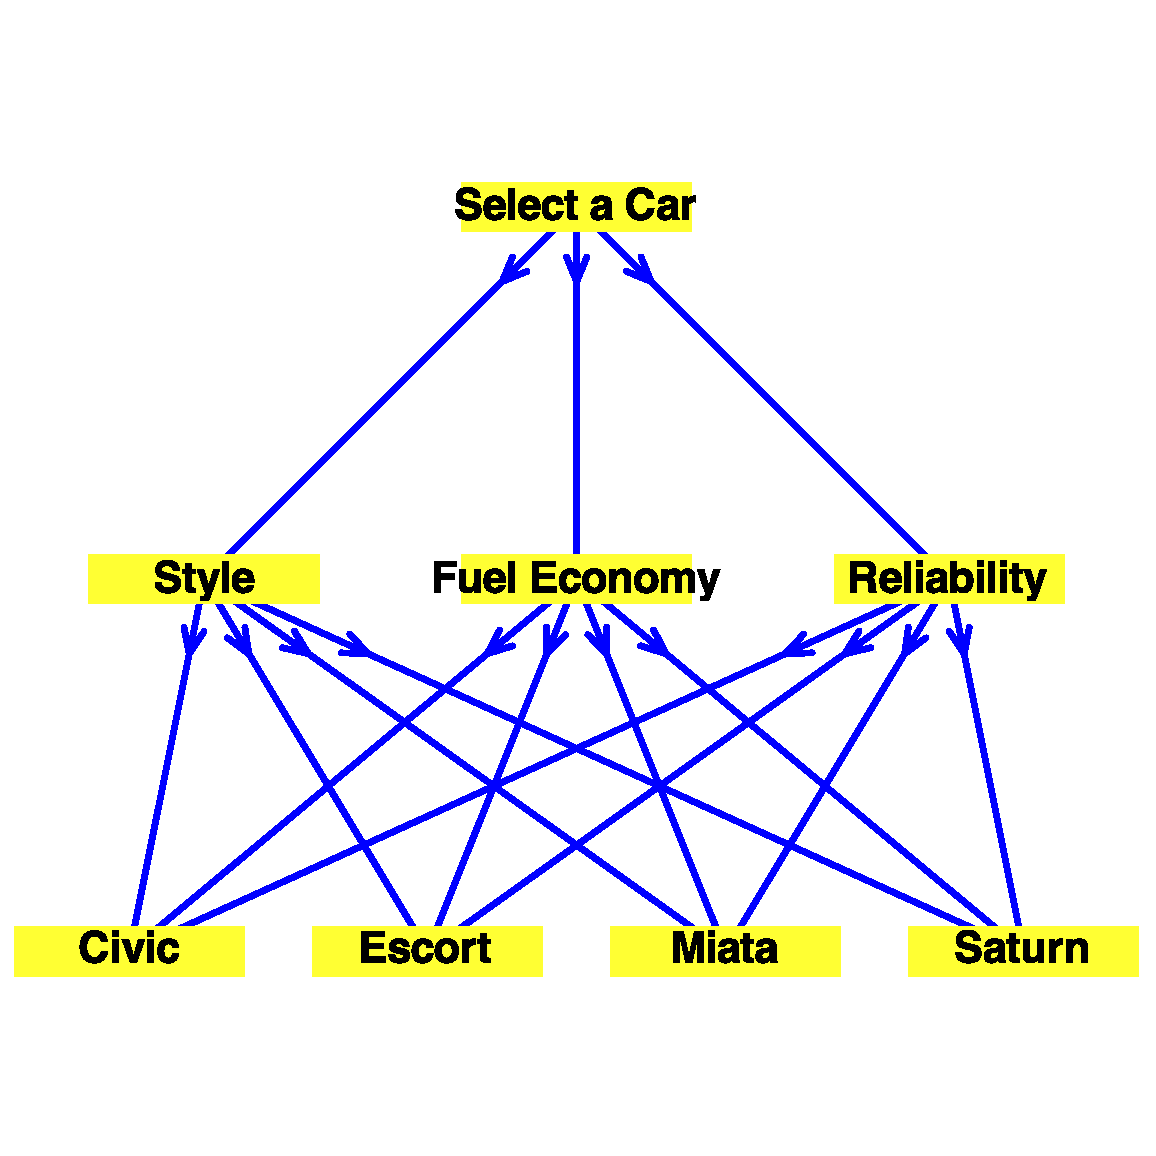
\includegraphics[width=0.75\textwidth]{TheCarGraph} \\[1ex]

\emph{Decision Hierarchy}
\end{center}
\end{frame}

%%%%%%
\begin{frame}[t,label=Criteria]
\frametitle{Pairwise Criteria Comparisons}
\vspace{-2ex}
{\small
\begin{block}{Compare...}
Using the scale \\[1ex]
\centerline{\footnotesize\fbox{\begin{tabular}{*{9}{@{\;\;}c}}
	{\it Criterion}$_1$ & & & & {\it versus} & & & &{\it Criterion}$_2$ \\[0.5ex]
	9 & 7 & 5 & 3 & 1 & 3 & 5 & 7 & 9 \\
	\hline
	extreme & very & strong & moderate & equal & moderate & strong & very & extreme \\[-0.5ex]
	importance & strong & 	    &   &  &  &  &  strong & importance
\end{tabular}}}
\vspace{1ex}
rate the relative importance of the criteria
\pause
to create a \href{http://mathsci.appstate.edu/~wmcb/Class/5340/ClassNotes141/AHP/Positive\%20Reciprocal\%20Matrix\%20Shiraishi\%2097.pdf}{\it positive reciprocal priority matrix}.
\vspace{-1ex}

\centerline{\renewcommand{\arraystretch}{1.5}%
\begin{tabular}{r | c c c}
	\multicolumn{1}{r}{\raisebox{10pt}{\rotatebox{-45}{over}}} & \multicolumn{1}{c}{Style} & Reliability & Fuel Economy \\
	\cline{2-4}
	Style & 1 & \fbox{\phantom{X}} & \fbox{\phantom{X}} \\
	Reliability & \rule[-2pt]{3ex}{0.5pt} & 1 & \fbox{\phantom{X}} \\
	Fuel Economy & \rule[-2pt]{3ex}{0.5pt} & \rule[-2pt]{3ex}{0.5pt} & 1
\end{tabular}}
\vspace*{1ex}
\pause
Now
\begin{enumerate}
\item Find\footnotemark\ the dominant eigenvalue $\lambda_m$. \quad\raisebox{-2pt}{\href{run:StartMaple.mw}{\beamergotobutton{\it Run Maple\ }}}
\pause
\item Find and normalize (so $\sum v_i=1$) $\lambda_m$'s eigenvector.
\end{enumerate}
\end{block}
\footnotetext{For Excel, c.f., the \href{http://college.cengage.com/mathematics/larson/elementary_linear/5e/students/ch08-10/chap_10_3.pdf}{\it power method} and the \href{http://en.wikipedia.org/wiki/Rayleigh_quotient_iteration}{\it Rayleigh quotient}.}
}
\end{frame}

%%%%%%
\begin{frame}
\frametitle{Pairwise Comparisons Chart}
\begin{center}
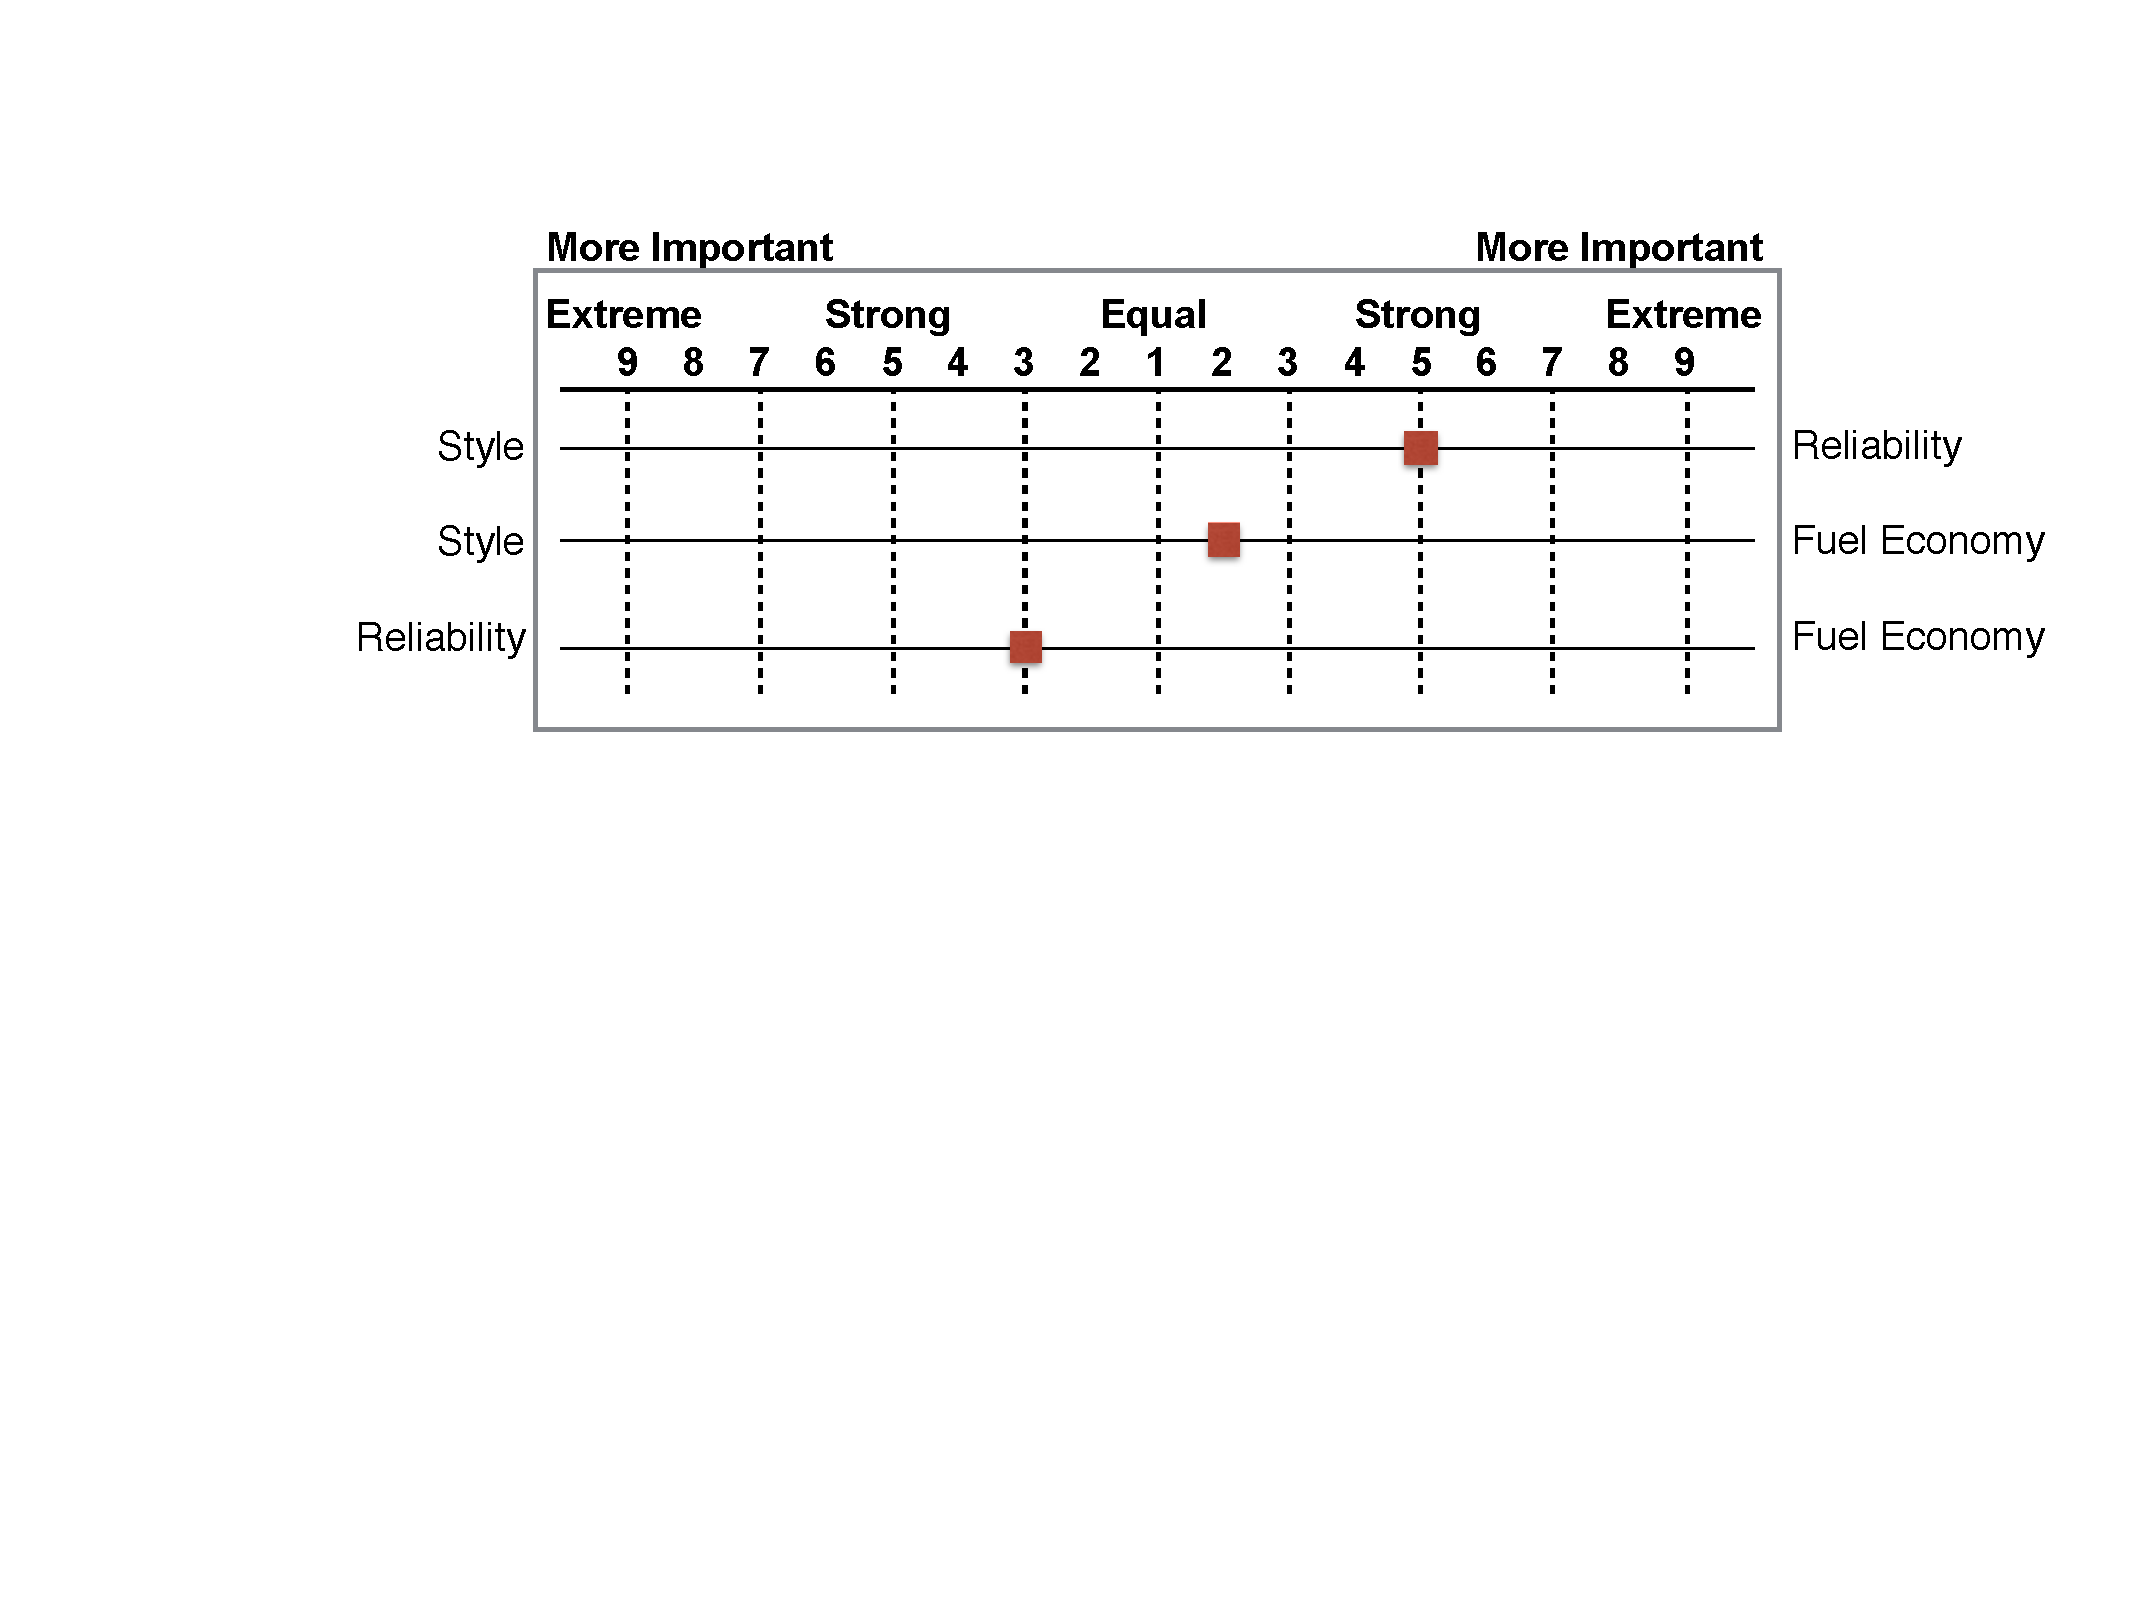
\includegraphics[width=.9\textwidth]{ComparisonChart}
\pause
\vspace{3ex}

\begin{tabular}{c@{\,}c}
	& $\begin{array}{ccc} S \  & R & \ FE \end{array}$ \\
  $\begin{array}{r} S \\ R \\ FE \end{array}$
	& $\begin{bmatrix}
	1 & 1/5 & 1/2 \\
	5 & 1	    & 3    \\
	2 & 1/3 & 1
	\end{bmatrix}$
\end{tabular} \quad \mbox{\phantom{XXX}}

\end{center}
\end{frame}

%%%%%%
\begin{frame}[t]
\frametitle{Pairwise Comparisons Eigenvector}
{\small
\vspace{-1.75ex}
\begin{block}{The Criteria Ranking}
The normalized eigenvector gives the relative ranking of the criteria.
\vspace{-1.5ex}
\[	\begin{array}{r} \text{Style} \\[1ex] \text{Reliability} \\[1ex] \text{Fuel Economy} \end{array} 
	= \begin{bmatrix} \\[-1.5ex] \fbox{\phantom{XXX}} \\[1ex] \fbox{\phantom{XXX}} \\[1ex] \fbox{\phantom{XXX}} \\[-1.5ex] \ \end{bmatrix}
	= ev_\text{\it Criteria}		\]
\end{block}
\pause
\vspace{-0.5ex}
\begin{block}{Consistency Index and Consistency Ratio}
Measure the consistency of the comparisons with the formulas
\vspace{-1ex}
\[	CI(\lambda_m) = \frac{\lambda_m - n}{n-1} \text{\qquad and\qquad} CR = CI(\lambda_m)/RI
	\vspace{-1ex}	\]
where $RI$ is from the following table listing \emph{random indices}. 
\vspace{1ex}

\centerline{\scriptsize\begin{tabular}{c | *{10}{c}}
$n$ & $3$ & $4$ & $5$ & $6$ & $7$ & $8$ & $9$ & $10$ \\
\hline
\parbox{18ex}{\strut \ Random Matrix \newline Consistency Index} & $0.52$ & $0.89$ & $1.11$ & $1.25$ & $1.35$ & $1.40$ & $1.45$ & $1.49$
\end{tabular}}
\vspace{1ex}
A ratio $CR < 0.1$ is good. {\scriptsize\it(Larger values mean the comparisons need revision.)}
\end{block}}
\end{frame}

%%%%%%
%%%%%%
\newsavebox\Chart
\savebox\Chart{%
\scriptsize\renewcommand{\arraystretch}{1.75}%
\begin{tabular}{r | c c c c}
	\multicolumn{1}{r}{\raisebox{7pt}{\rotatebox{-45}{over}}\hspace*{-1.5ex}} & \multicolumn{1}{c}{Civic} & Saturn & Escort & Miata \\
	\cline{2-5}
	Civic & 1 & \fbox{\phantom{X}} & \fbox{\phantom{X}} & \fbox{\phantom{X}} \\
	Saturn & \rule[-2pt]{3ex}{0.5pt} & 1 & \fbox{\phantom{X}} & \fbox{\phantom{X}} \\
	Escort &\rule[-2pt]{3ex}{0.5pt} & \rule[-2pt]{3ex}{0.5pt}  & 1 & \fbox{\phantom{X}} \\
	Miata & \rule[-2pt]{3ex}{0.5pt} & \rule[-2pt]{3ex}{0.5pt} & \rule[-2pt]{3ex}{0.5pt} & 1 \\
\end{tabular}}
%%%%%%
%%%%%%

%%%%%%
\begin{frame}[t,label=Alternatives]
\frametitle{Pairwise Alternatives Comparisons}
\begin{block}{Alternatives Comparisons}
For each criterion, construct the pairwise comparison matrix \\[2ex]

\centerline{\begin{tabular}{@{}c |@{} c}
\emph{Style}	& \emph{Reliability} \\
\usebox{\Chart} & \usebox{\Chart} \\[9ex]
\pause
\  $ev_S = \begin{bmatrix} \fbox{\phantom{XX}}, \fbox{\phantom{XX}}, \fbox{\phantom{XX}}, \fbox{\phantom{XX}} \end{bmatrix}$ &
	$ev_R = \begin{bmatrix} \fbox{\phantom{XX}}, \fbox{\phantom{XX}}, \fbox{\phantom{XX}}, \fbox{\phantom{XX}} \end{bmatrix}$
\end{tabular}}
\vspace{3ex}
\pause

\emph{Fuel Economy} is an objective value; it needs no comparison matrix. Normalize so the sum is $1$ and use for its `eigenvector':
\vspace{-1ex}
\[	\left[34, \ 27, \ 24, \ 28\right] \implies	ev_{FE} = \left[ 0.30, \ 0.24, \ 0.21, \ 0.25 \right]	\]
\end{block}
\end{frame}

%%%%%%
\begin{frame}[t,label=TheRanking]
\frametitle{Comparison Matrix}
\begin{block}{AHP Comparison Matrix}
\begin{itemize}
\item Form the \emph{comparison matrix} from the eigenvectors
\vspace{-1ex}
{\footnotesize
\[	CM = \left[ ev_S, \ ev_R, \ ev_{FE}\right] = \begin{bmatrix}
		\begin{bmatrix} \fbox{\phantom{XX}} \\[0.75ex] \fbox{\phantom{XX}} \\[0.75ex] \fbox{\phantom{XX}}\\[0.75ex] \fbox{\phantom{XX}}  \end{bmatrix}
	     & \begin{bmatrix} \fbox{\phantom{XX}} \\[0.75ex] \fbox{\phantom{XX}} \\[0.75ex] \fbox{\phantom{XX}}\\[0.75ex] \fbox{\phantom{XX}}  \end{bmatrix}
	     & \begin{bmatrix} \fbox{\phantom{XX}} \\[0.75ex] \fbox{\phantom{XX}} \\[0.75ex] \fbox{\phantom{XX}}\\[0.75ex] \fbox{\phantom{XX}}  \end{bmatrix}
	\end{bmatrix}	\]
}
\pause

\item Multiply the comparison matrix by the eigenvector of priority rankings for the criteria $\vec{R}=CM \cdot ev_\text{\it Criteria}$ to produce the \emph{rankings vector} $\vec{R}$
\[	R = \begin{bmatrix} \fbox{\phantom{XX}} & \fbox{\phantom{XX}} & \fbox{\phantom{XX}} & \fbox{\phantom{XX}} \end{bmatrix}
	\vspace{-1ex}	\]
\pause

\item To include \emph{cost}: 
	\begin{enumerate}
	\item Normalize the cost vector so the sum is 1. 
	\item Divide respective rankings by cost to generate the \emph{cost-benefit vector}.
	\end{enumerate}
\end{itemize}
\end{block}
\end{frame}

%%%%%%
\begin{frame}[label=FlowChart]
\frametitle{AHP Workflow Charts}
{\scriptsize
\begin{columns}[c]
      \begin{column}{0.45\textwidth}
	\centerline{\includegraphics[width=1.1\textwidth]{AHPWorkflow}}
	\vspace{4ex}
	
	\parbox{\textwidth}{From: T.~L.~Saaty, ``\href{http://mathsci2.appstate.edu/~wmcb/Class/5340/ClassNotes141/AHP/Analytic\%20Hierarchy\%20Proc\%20Saaty\%202008.pdf}{Decision making with the analytic hierarchy process},'' \href{http://www.inderscience.com/info/inarticletoc.php?jcode=ijssci&year=2013&vol=5&issue=1}{Int.~J.~Services Sciences}, Vol.~1, No.~1, 2008. Figure 2, pg.~94.}
	\vfill
      \end{column}
      \pause
      \begin{column}{0.55\textwidth}
      	\hspace*{-10ex}\parbox{1.125\textwidth}{%
	\begin{description}
	\item[Step 1]  Create the decision hierarchy by breaking the decision problem into interrelated decision elements
	\item[Step 2]  Collect input data with pairwise comparisons of decision elements
	\item[Step 3]  Use eigenvalues to estimate the relative weights of decision elements
	\item[Step 4]  Aggregate the relative weights of decision elements to rate the decision alternatives \\[9.5ex]
	\end{description}}
	\vfill
	From: F.~Zahedi, ``\href{http://www.jstor.org/stable/25060854}{The Analytic Hierarchy Process: A~Survey of the Method and Its Applications},'' 
	\href{http://pubsonline.informs.org/toc/inte/current}{\emph{Interfaces}}, Vol.~16, No.~4 (Jul-Aug, 1986), pg.~96.
      \end{column}
\end{columns}
\vfill
\centerline{\href{run:AHP Spreadsheet.xlsx}{\beamergotobutton{\it Open Excel Example}}}
}
\end{frame}

%%%%%%
\begin{frame}[label=MultipleAssessments]
\frametitle{Combining Multiple Assessments}
\begin{block}{Assessments from Multiple Agents: First Method}
\vspace{0.75ex}
\begin{enumerate}
\setlength{\itemsep}{2ex}
\item Each individual ranks all pairs of criteria.
\pause
\item Average the rankings with a \href{http://en.wikipedia.org/wiki/Geometric_mean}{\it geometric mean}\footnotemark.
\pause
\item Create the positive reciprocal priority matrix from the geometric means of the rankings.\newline
	{\it \footnotesize (Unlike arithmetic means, geometric means preserve reciprocals.)}
\pause
\item Follow the same procedure with each individual ranking each of the alternatives.
\pause
\item Use the matrices of geometric means in AHP. 
\vspace{0.75ex}
\end{enumerate}
\end{block}
\footnotetext{See \href{http://www.maa.org/sites/default/files/gwan01200422828.pdf}{The HM-GM-AM-QM Inequalities} by P.~Gwanyama}
\end{frame}

%%%%%%
\begin{frame}
\frametitle{Combining Multiple Assessments, II}
\begin{block}{Assessments from Multiple Agents: Second Method}
\begin{enumerate}
\item Each agent completes an AHP producing their final ranking
\item Use the geometric mean of the individual final rankings to create an overall final ranking.
\end{enumerate}
\end{block}
\pause
\vfill

\begin{block}{Assessments from Multiple Agents: Third Method}
\begin{enumerate}
\item Each agent completes an AHP producing their final ranking
\item If the individual criteria priority matrices are very different, raise the final ranking to the power of the criteria priorities.
\item Use the geometric mean of the individual, power-adjusted, final rankings to create an overall final ranking.
\end{enumerate}
\end{block}
\vfill
\centerline{\small Hundereds of examples are in \href{http://books.google.com/books?id=c8KqSWPFwIUC&lpg=PT331&dq=The\%20Hierarchon\%3A\%20A\%20Dictionary\%20of\%20Hierarchies&pg=PT331\#v=onepage&q&f=false}{\it The Hierarchon:~A Dictionary of Hierarchies} by Saaty.}
\end{frame}

%%%%%%
\begin{frame}
\frametitle{Combining Multiple Assessments Example}
\vspace{-1ex}
{\small
\begin{block}{Simple Example}
Given three assessment matrices 
\vspace{-1ex}
\[	PM1 = \begin{bmatrix} 1&2&3 \\ 1/2&1&1/4 \\ 1/3&4&1 \end{bmatrix}, 
	\quad PM2 = \begin{bmatrix} 1&3&1/2 \\ 1/3&1&2 \\ 2&1/2&1 \end{bmatrix},
	\quad PM3 = \begin{bmatrix} 1&1/2&5 \\ 2&1&3 \\ 1/5&1/3&1 \end{bmatrix},
	\vspace{-1ex}	\]
\pause

form the assessment matrix $PM=[pm_{i,j}]$ with 
\[	pm_{i,j}=\operatorname{GeometricMean}(PM1_{i,j},PM2_{i,j},PM3_{i,j})	\]
\[	PM = \begin{bmatrix} 1&\sqrt[3]{3}& \sqrt[3]{\frac{15}{2}}\; \\[0.75ex]
		\sqrt[3]{\frac{1}{3}} &1& \sqrt[3]{\frac{3}{2}} \\[0.75ex] 
		\sqrt[3]{\frac{2}{15}} & \sqrt[3]{\frac{2}{3}} &1 \end{bmatrix} 
	\approx \begin{bmatrix} 1.0& 1.44& 1.96 \\ 0.693& 1.0& 1.14 \\ 0.511 & 0.872& 1.0 \end{bmatrix}	\]
\pause
\vspace{2ex}

The critical property of geometric means needed is
\vspace{-1ex}
\[	\operatorname{GeometricMean}(1/x_i) = 1/ \operatorname{GeometricMean}(x_i).	\]
\end{block}
}
\end{frame}

%%%%%%
\begin{frame}[label=axioms]
\frametitle{Axioms of the Analytic Hierarchy Process}
\begin{block}{The Basic Principle of AHP{\normalfont\footnotemark}}
\begin{description}
\item[Principle of Hierarchic Composition.] Multiply local priorities of elements in a cluster by the ``global'' priority of the parent element producing global priorities throughout the hierarchy.
\end{description}
\end{block}
\pause
\vfill
\begin{block}{The Axioms of AHP}
\begin{description}
\setlength{\itemsep}{2ex}
\item[Reciprocal Axiom]  If $P(A,B)$ is the paired comparison of $A$ to $B$, then $P(B,A)=1/P(A,B)$.
\pause
\item[Homogeneity Axiom]\hspace{-3pt}  Elements being compared do not differ by \emph{too much}.\newline\mbox{} \hfill {\it\footnotesize(Over an order of magnitude leads to judgment errors.)}
\pause
\item[Synthesis Axiom] Judgments about the priorities of the elements in a hierarchy do not depend on lower level elements.
\end{description}
\end{block}
\vfill
\footnotetext{See ``\href{http://www.jstor.org/discover/10.2307/3088581?uid=3739256&uid=2&uid=4&sid=21103790751913}{The Analytic Hierarchy Process:~An Exposition},''  Forman \& Gass, \emph{Operations Research}, Vol. 49, No. 4 (Jul.~- Aug., 2001), pp.~469-486.}
\end{frame}

%%%%%% Appendix
%%%%%%
\begin{frame}[label=PowerMethod]
\frametitle{The Power Method for the Maximal Eigenvector}
\begin{block}{Power Method\footnotemark}
Suppose that $\mathbf{M}$ is a square matrix that has a dominant eigenvalue $|\lambda_1| > |\lambda_i|$ for $i=2...$

\begin{enumerate}
\item Choose $\vec{x}_0 \ne \vec{0}$. \quad {\footnotesize In AHP, we normally use $\vec{x}_0=\langle1,1,1\rangle$}
\item Compute the ``scaled power sequence''
	\vspace{-2ex}
	\begin{align*}\footnotesize
		\vec{x}_1 &= \tfrac{1}{\ \|\mathbf{M}\cdot\vec{x}_0\|_\infty}\cdot \mathbf{M}\cdot\vec{x}_0 \\
		\vec{x}_2 &= \tfrac{1}{\ \|\mathbf{M}\cdot\vec{x}_1\|_\infty}\cdot \mathbf{M}\cdot\vec{x}_1 
			= \tfrac{1}{\ \|\mathbf{M}\cdot\vec{x}_1\|_\infty\cdot \|\mathbf{M}\cdot\vec{x}_0\|_\infty}\cdot \mathbf{M}^2\cdot\vec{x}_0 \\
		\vec{x}_3 &= \tfrac{1}{\ \|\mathbf{M}\cdot\vec{x}_2\|_\infty}\cdot \mathbf{M}\cdot\vec{x}_2 
			= \tfrac{1}{\ \|\mathbf{M}\cdot\vec{x}_2\|_\infty\cdot \|\mathbf{M}\cdot\vec{x}_1\|_\infty\cdot \|\mathbf{M}\cdot\vec{x}_0\|_\infty}\cdot \mathbf{M}^3\cdot\vec{x}_0 \\[-2ex]
			&\ \,\vdots \\[-5ex]
	\end{align*}
\item Continue the sequence until $\|\vec{x}_{k+1} - \vec{x}_k\| <\varepsilon$.
\end{enumerate}
\end{block}
\footnotetext{See also ``\href{http://en.wikipedia.org/wiki/Power_iteration}{Power Iteration}'' on Wikipedia.}
\end{frame}

%%%%%%
\begin{frame}[label=Rayleigh]
\frametitle{The Rayleigh Quotient for the Maximal Eigenvalue}
\begin{block}{The Rayleigh Quotient\footnotemark}
Let $\vec{x}$ be a nonzero vector and $\mathbf{M}$ be a square matrix. Define the \emph{Rayleigh quotient of $\vec{x}$} to be
\[	R(\vec{x}) = \frac{\vec{x} \cdot (\mathbf{M}\cdot\vec{x}\,)}{\vec{x}\cdot\vec{x}}	\]
If $\vec{x}$ is an eigenvector, then $\mathbf{M}\cdot\vec{x} = \lambda\vec{x}$, so $R(\vec{x})$ simplifies to $\lambda$, the eigenvalue of the eigenvector $\vec{x}$. 
\end{block}
\vfill

\begin{block}{Estimating the Maximal Eigenvalue}
Let $\{\vec{x}_k\}$ be vectors generated via the power method and set $r_k=R(\vec{x}_k)$.
\vspace{1ex}

If $\vec{x}_k \to \vec{x}$, the dominant eigenvector, then $r_k\to \lambda$ the eigenvalue of $\vec{x}$.
\vspace{2ex}

{\footnotesize (Nota bene: $\mathbf{M}\cdot\vec{x}_k \ne \vec{x}_{k+1}$. The $\vec{x}_{k}$s are scaled.)}
\end{block}
\vfill
\footnotetext{See also ``\href{http://en.wikipedia.org/wiki/Spectral_radius}{Spectral Radius}'' on Wikipedia.}
\end{frame}


%%%%%%
\end{document}
\end
